\documentclass[10pt,a4paper]{article}
\usepackage[utf8]{inputenc}
\usepackage{amsmath}
\usepackage{amsfonts}
\usepackage{amssymb}
\usepackage{graphicx}
\usepackage{subcaption}
\title{Heightmap correction}
\begin{document}
\section{The data}
Each image is associated with a height map, which has been retrieved by applying \texttt{} to the actin channel (currently- check what the analysis was at the time of anayzing Exp0168).  Pixels in the 2D image are taken from the height indicated in the height map.  

In Experiment0168, height variations are small (\textbf{missing: voxel dimension metadata}); in confocal experiments there will be large steps in height difference.

\begin{figure}
\begin{subfigure}{\textwidth}
\centering
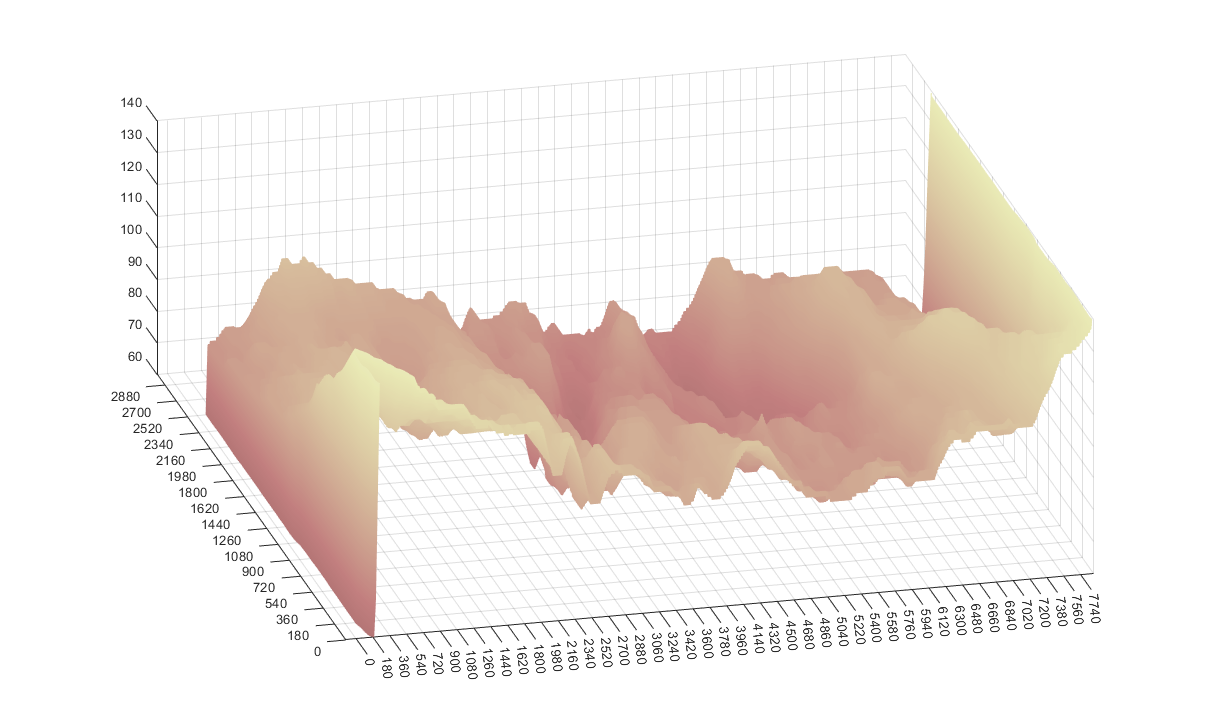
\includegraphics[width=\textwidth]{435_example2.png}
\subcaption{Exaggerated view, note stretched z-axis.}
\end{subfigure}
\begin{subfigure}{\textwidth}
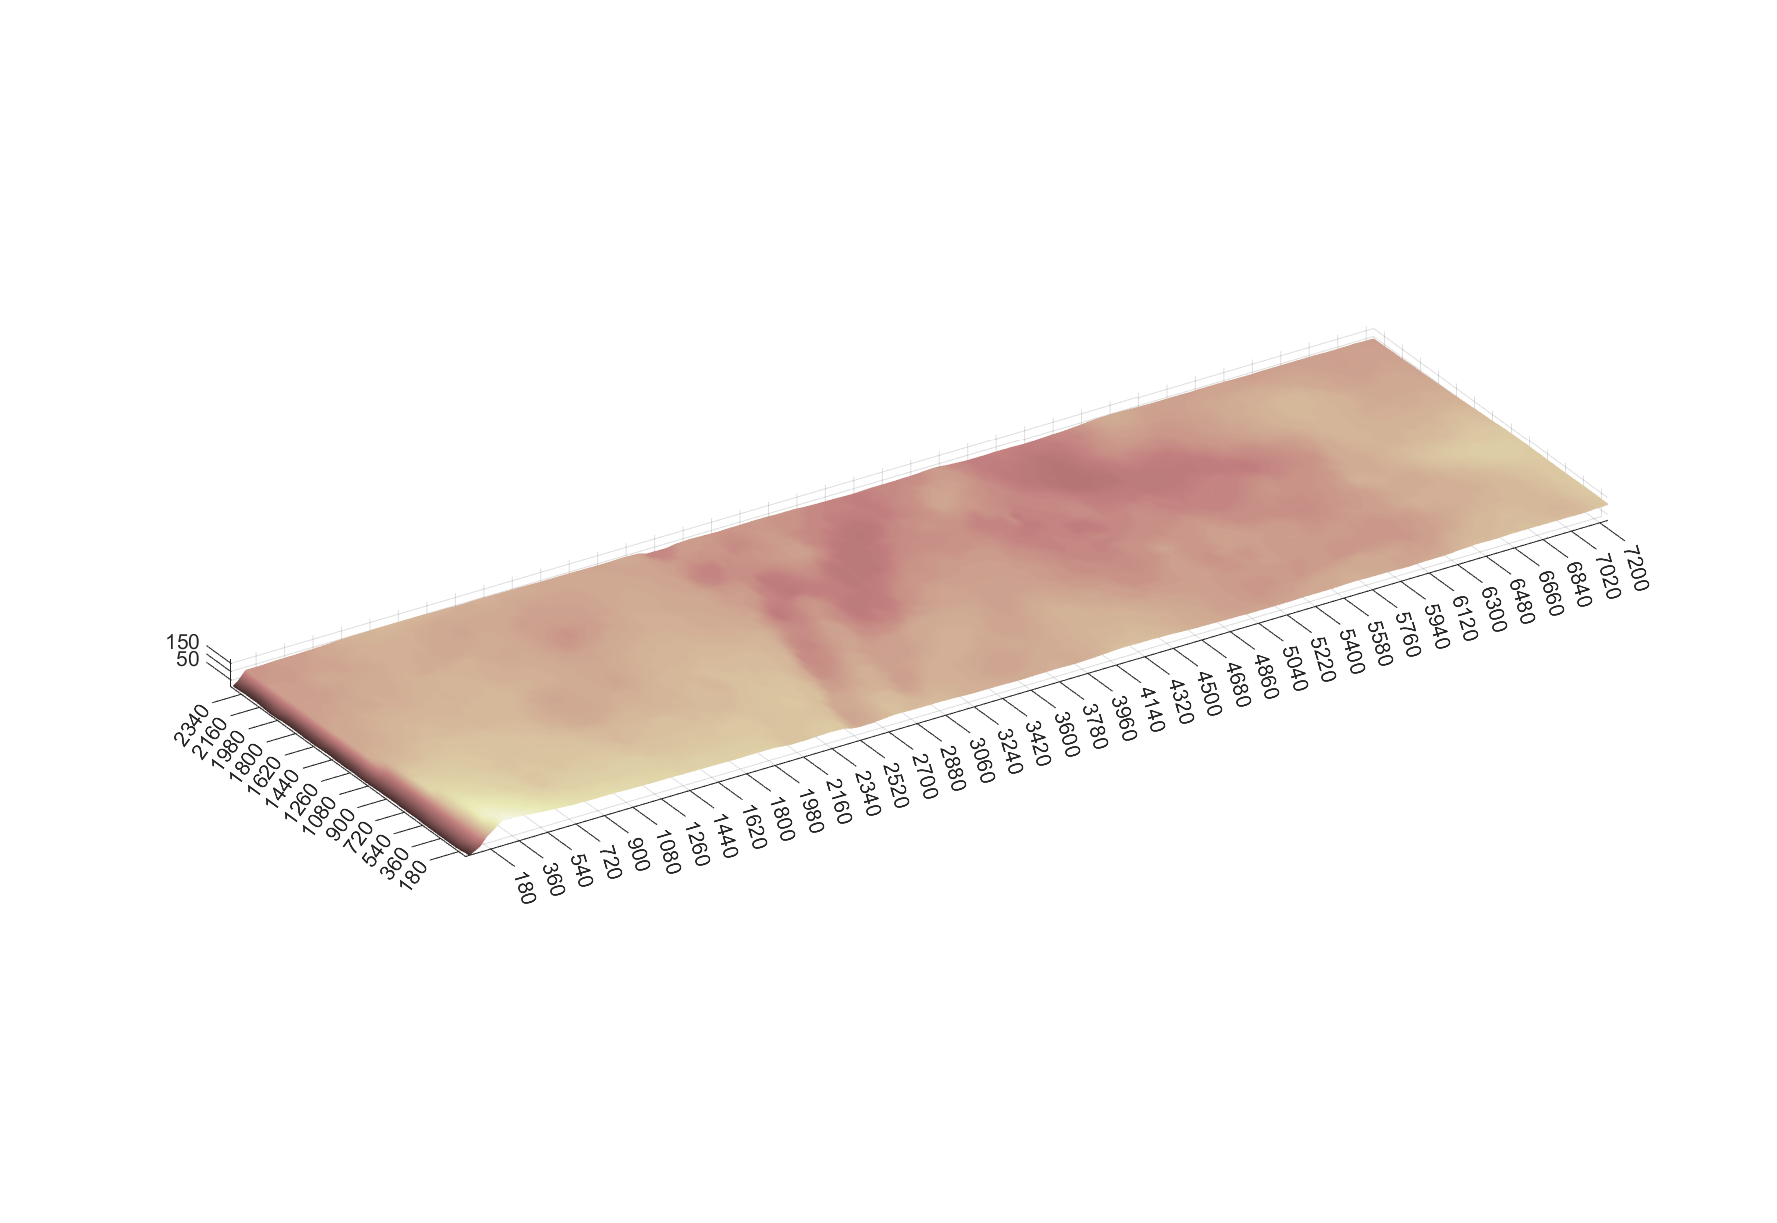
\includegraphics[width=\textwidth]{435_flat.png}
\subcaption{Realistic scaling, assuming cubic voxels}
\end{subfigure}
\caption{Height map from time 435 in experiment 0168: a severely curved heightmap from late in the experiment.  Scaling of axes to scale.  The grid increments show $180 \times 180$ squares, scale of tiles in the Fourier space analysis for myosin orientation.}
\end{figure}
\section{Initial smoothing?}
I don't want to correct distances for pixel-scale height fluctuations at less than cell-scale - this would wrongly inflate the area of each cell.  On option is too smooth the heightmap prior to any processing (Gaussian filter).  While its ok if steps in height become distributed over the neighboring pixels within a tile, height differences should remain localized to their tile.  The step is especially relevant in the case of confocal data with poor z-resolution: sudden steps with localized high slope can be smoothed to gentler gradients.  (Is it in fact more realistic to regard the height step as possible de-localized over a tile edge?  Does this better approximate the expected height profile of the epithelial layer?)

Another option is too average / coarsen some derived quantity such as metric over tiles.

A plane could be fitted to approximate the height profile of each tile - see Gaussian curvature conservation section below.

\section{Metric and curvature (pixel scale)}
The data represents a graph above a plane.  Monge geometry applies.  The metric tensor/ first fundamental form can be calculated as.

\begin{equation}
g =  \begin{pmatrix}
1+(\partial_x f) ^2 &&\partial_x f \partial_y f \\
\partial_y f \partial_x f && 1+ (\partial_y f)^2\\
\end{pmatrix}
\end{equation}

\begin{equation}
\begin{aligned}
\sqrt{|g|} &=  \sqrt{(1 + (\partial_x f)^2)(1 + (\partial_y f)^2)-(\partial_x f \partial_y f)^2}\\
&\approx \sqrt{1 + (\partial_x f)^2 + (\partial_y f)^2}
\end{aligned}
\end{equation}

Here $\partial_x f$, $\partial_y f$ were taken using the implementation of numerical derivative in matlab \texttt{gradient}, a central difference $\partial_x f = \frac{f_{i+1}-f_{i-1}}{2}$.  Could have used \texttt{diff} for backwards/forwards differences.

\begin{figure}
\caption{Metric determinant $\sqrt{g}$, indicating relative area represented by each pixel.}
\end{figure}

For curvature tensor/ second fundamental form, second derivatives are needed.  I use \texttt{diff} twice to implement numerical second derivatives

Gaussian curvature

Mean curvature
\subsection{Conservation of Gaussian curvature}
Total Gaussian curvature of a plane with constant boundary should be a constant.  If pixel-scale height map is coarsened to a tile-scale height mesh, Gaussian curvature will be concentrated in the vertices, where it will be lost to subsequent analysis.  However, since tiles are overlapping, we have a `disjointed' mesh of tiles and gaussian curvature is not conserved.
\section{Result}
\subsection{Exp0168}
(Voxel dimension metadata needed - assuming voxels are cubic)

Height steps are by 1 pixel.  Aggregate height differences are small compared to in-plane distances, see Fig 1.

Some pixels are up to $1.1 \times$ bigger than other ones.  Based on just experiment 0168, it might not be worth correcting for this... ??  

TODO Unclear how strongly nonlinear derived quantities are affected by this slight distortion.

There are no problems with sub-cell-scale height fluctuations.

\section{Fourier transform approach}
\subsection{Tile level}
Smoothing the height map to tile level, each tile is approximated as a stretched and sheared rectangle.  Height variations and the associated distortions in projected lengths within each tile are ignored.  This is valid if the lengthscale of height variations is greater than tile scale.  
\subsection{Mean metric?}
\section{Anisotropy}
Up to fitting an ellipse/measuring an inertia matrix in Fourier space and transforming back, the skewing and stretchign operation commutes and can equivalently be performed after the Fourier transform steps.  However, the final result, local anisotropy indicators \texttt{t} and \texttt{angS} are nonlinear (log) functions of the inertia matrix / fitted ellipse and can't simply be (un-)stretched.  For the ellipse-fitting method, 
\begin{equation}
S = 1/2 \log(L_{maj}/L_{min});
\end{equation}
major and minor axes $L_{maj}$ and $L_{min}$ of the fitted ellipse in real space can be adjusted to account for the projection by a factor such as $\sqrt{h_{xx}}/\sqrt{h_{yy}}$.  Equivalently 
\begin{equation}
S_{curv} = 1/2 \left( \log(L_{maj}/L_{min}) + \log(\mathtt{ratiocorrection}) \right);
\end{equation}
\section{Is the height map the epithelial surface?}
If the height map cuts through the epithelial layer diagonally, cell areas and anisotropies will be artificially inflated by `correcting' the projection.

Don't overcorrect for height fluctuations smaller than cell scale!  This would artificially inflate cell areas everywhere.

What scale and smoothness of height map is realistic?  The initial height map should conform to our expectations of profile of the epithelial surface, or as close as possible in a discretized way in the case of confocal data with poor z-resolution.
\end{document}